\renewcommand{\theequation}{5.\arabic{equation}}
\begin{enumerate}[label=(\alph*)]
\item
Vì tất cả các thanh có cùng bề dày theo phương vuông góc mặt phẳng bài toán, nên khi lấy tỉ số các đại lượng hình học, thừa số bề dày triệt tiêu và có thể bỏ qua. Xét hệ chưa nhận nhiệt, đường cao của hình thang:
\begin{equation}
  h_0=\sqrt{L_2^2 - \left(\frac{L_3-L_1}{2}\right)^2}
\end{equation}

Sau khi nhận nhiệt, độ dài các thanh là:
\begin{equation}
\begin{aligned}
  \text{Thanh AB}:\quad &L'_1=L_1 \text{ (không nở vì nhiệt)},\\
  \text{Thanh CD}:\quad &L'_3=L_3+\Delta L_3=L_3(1+\alpha_3\Delta T),\\
  \text{Thanh AD và BC}:\quad &L'_2=L_2+\Delta L_2=L_2(1+\alpha_2\Delta T).
\end{aligned}
\end{equation}

Đường cao mới của hình thang (bỏ qua phần tử $\Delta T^2$ rất nhỏ):
\begin{equation}
  \begin{aligned}
  h'&=\sqrt{{L'_2}^2-\left(\frac{{L'_3}-{L'_1}}{2}\right)^2}\\
    &=\sqrt{L_2^2(1+\alpha_2\Delta T)^2-\left(\frac{L_3(1+\alpha_3\Delta T)-L_1}{2}\right)^2}\\
    &\approx \sqrt{L_2^2(1+2\alpha_2\Delta T)-\left[\left(\frac{L_3-L_1}{2}\right)^2+\frac{(L_3-L_1)L_3\alpha_3\Delta T}{2}\right]}\\
    &=\left(h_0^2+2L_2^2\alpha_2\Delta T-\frac{(L_3-L_1)L_3\alpha_3\Delta T}{2}\right)^{1/2}\\
    &\approx h_0+\frac{1}{2h_0}\left(2L_2^2\alpha_2\Delta T-\frac{(L_3-L_1)L_3\alpha_3\Delta T}{2}\right)
  \end{aligned}
\end{equation}

Độ biến thiên chiều cao:
\begin{equation}
\begin{aligned}
  \Delta h = h'-h_0 &= \frac{1}{2h_0}\left(2L_2^2\alpha_2\Delta T-\frac{(L_3-L_1)L_3\alpha_3\Delta T}{2}\right) \\
  &=\frac{4L_2^2\alpha_2 - L_3(L_3-L_1)\alpha_3}{4h_0} \Delta T \\
  &= \frac{4L_2^2\alpha_2-L_3(L_3-L_1)\alpha_3}{4\left(L_2^2-\left(\frac{L_3-L_1}{2}\right)^2\right)^{1/2}}\Delta T
\end{aligned}
\end{equation}

Hệ số nở nhiệt hiệu dụng theo phương thẳng đứng của hình thang: 
\begin{equation}
\begin{aligned}
  \alpha_{eff}=\frac{\Delta h}{h_0\Delta T}&=\frac{4L_2^2\alpha_2 - L_3(L_3-L_1)\alpha_3}{4h_0^2} \\
  &=\frac{16L_2^2\alpha_2-4L_3(L_3-L_1)\alpha_3}{16L_2^2-(L_3-L_1)^2}
\end{aligned}
\end{equation}

Trạng thái của hệ phụ thuộc vào hệ số nở nhiệt hiệu dụng của hệ:
\begin{equation}
\begin{cases}
  \alpha_{eff}>0 \Leftrightarrow \dfrac{\alpha_2}{\alpha_3}>\dfrac{L_3(L_3-L_1)}{4L_2^2}, & \text{hệ nở chiều cao},\\[3mm]
  \alpha_{eff}<0 \Leftrightarrow \dfrac{\alpha_2}{\alpha_3}<\dfrac{L_3(L_3-L_1)}{4L_2^2}, & \text{hệ co chiều cao},\\[3mm]
  \alpha_{eff}=0 \Leftrightarrow \dfrac{\alpha_2}{\alpha_3}=\dfrac{L_3(L_3-L_1)}{4L_2^2}, & \text{hệ không đổi chiều cao}.
\end{cases}
\end{equation}

\item
Xét cấu trúc hình thang. Diện tích hình thang ban đầu được cho bởi:
\begin{equation}
S=\frac{1}{2}(L_1+L_3)h_0
\end{equation}

Sau khi tăng nhiệt độ $\Delta T$, diện tích mới (bỏ qua số hạng bậc cao $\Delta h \Delta T \propto \Delta T^2$) là:
\begin{equation}
\begin{aligned}
  S'&=\frac{1}{2}(L_1'+L_3')h' \\
  &=\frac{1}{2}\left[L_1+L_3(1+\alpha_3\Delta T)\right](h_0+\Delta h) \\
  &\approx \frac{1}{2}\left[(L_1+L_3)h_0 + (L_1+L_3)\Delta h + L_3\alpha_3 h_0 \Delta T\right]
\end{aligned}
\end{equation}

Tỉ số giữa diện tích lúc sau và diện tích ban đầu :
\begin{equation}
\begin{aligned}
  \frac{S'}{S} &\approx 1 + \frac{\Delta h}{h_0} + \frac{L_3\alpha_3}{L_1+L_3}\Delta T \\
  &= 1 + \left(\alpha_{eff} + \frac{L_3\alpha_3}{L_1+L_3}\right)\Delta T
\end{aligned}
\end{equation}

Do độ dày vuông góc với mặt giấy của các thanh là như nhau và không đổi, tỉ số thể tích bằng tỉ số diện tích:
\begin{equation}
\begin{aligned}
  \frac{V'}{V} = \frac{S'}{S} &\approx 1 + \left( \frac{16L_2^2\alpha_2-4L_3(L_3-L_1)\alpha_3}{16L_2^2-(L_3-L_1)^2} + \frac{L_3\alpha_3}{L_1+L_3} \right)\Delta T \\
  &= 1 + \left[ \frac{16L_2^2(L_1+L_3)\alpha_2 + L_3(16L_2^2 - 5L_3^2 + 2L_1L_3 + 3L_1^2)\alpha_3}{(L_1+L_3)\left[16L_2^2-(L_3-L_1)^2\right]} \right]\Delta T
\end{aligned}
\end{equation}

\item
Ta có thể chia hệ thành một khối lập phương cạnh $L$ được gắn với 6 hình chóp cụt tứ giác đều ở các mặt. Khi hệ chưa nhận nhiệt, chiều cao ban đầu của hình chóp cụt: 
\begin{equation}
 h_0=\sqrt{b^2 - \frac{[\sqrt{2}(L-a)]^2}{4}}=\sqrt{b^2 - \frac{(L-a)^2}{2}}
\end{equation}

Thể tích hình chóp cụt tứ giác đều là:
\begin{equation}
  V_0=\frac{1}{3}h_0 \left( L^2 +a^2 + \sqrt{L^2 a^2} \right)= \frac{1}{3}h_0 \left( L^2 +a^2 + aL \right)
\end{equation}
Thể tích của cả hệ ban đầu:
\begin{equation}
\begin{aligned}
  V&=6V_0+L^3\\
  &=2h_0(L^2 +a^2 + aL) + L^3
\end{aligned}
\end{equation}

Khi hệ nhận nhiệt, chiều dài các cạnh biến đổi thành:
\begin{equation}
\begin{aligned}
  \text{Cạnh khối lập phương}:\quad L'&=L \text{ (không nở vì nhiệt)},\\
  \text{Cạnh tấm vuông}:\quad a'&=a+\Delta a \\ 
  &=a(1+\alpha_1\Delta T) \implies a'^2 \approx a^2(1+ 2\alpha_1 \Delta T),\\
  \text{Cạnh nối}:\quad b'&=b+\Delta b \\
  &=b(1+\alpha_2\Delta T) \implies b'^2 \approx b^2(1+ 2\alpha_2 \Delta T).
\end{aligned}
\end{equation}

Chiều cao hình chóp sau khi nhận nhiệt:
\begin{equation}
\begin{aligned}
  h' &= \sqrt{{b'}^2 - \frac{(L'-a')^2}{2}} \\
  &\approx \sqrt{b^2(1+ 2\alpha_2 \Delta T) - \frac{L^2-2aL(1+\alpha_1\Delta T)+a^2(1+ 2\alpha_1 \Delta T)}{2}} \\
  &= \sqrt{b^2-\frac{(L-a)^2}{2}+2b^2 \alpha_2 \Delta T+aL \alpha_1 \Delta T-a^2\alpha_1 \Delta T} \\
  &= \left[ h_0^2+\left(2b^2 \alpha_2 +aL \alpha_1 -a^2\alpha_1\right) \Delta T \right]^\frac{1}{2}\\ 
  &\approx h_0+\frac{2b^2\alpha_2+aL\alpha_1-a^2\alpha_1}{2h_0}\Delta T
\end{aligned}
\end{equation}

Độ biến thiên chiều cao:
\begin{equation}
\begin{aligned}
  \Delta h &= h'-h_0\\ 
  &=\frac{2b^2\alpha_2+aL\alpha_1-a^2\alpha_1}{2h_0}\Delta T
\end{aligned}
\end{equation}

Thể tích lúc sau của một hình chóp cụt:
\begin{equation}
\begin{aligned}
  V_0'&=\frac{1}{3}h' \left( {L'}^2 + {a'}^2 + L'a' \right) \\
  &\approx \frac{1}{3}\left(h_0 + \Delta h\right)\left[L^2 + a^2(1+ 2\alpha_1 \Delta T) + aL(1+\alpha_1\Delta T)\right] \\
  &\approx V_0 + \frac{1}{3}h_0(2a^2+aL)\alpha_1\Delta T + \frac{1}{3}(L^2+a^2+aL)\Delta h
\end{aligned}
\end{equation}

Thể tích toàn hệ lúc sau:
\begin{equation}
\begin{aligned}
  V'&=6V_0'+L^3 \\
  &=6V_0+2h_0(2a^2+aL)\alpha_1\Delta T + 2(L^2+a^2+aL)\Delta h +L^3
\end{aligned}
\end{equation}

Tỉ số giữa thể tích lúc sau và lúc đầu:
\begin{equation}
\label{eq5:c1}
\begin{aligned}
  \frac{V'}{V} &= \frac{6V_0+2h_0(2a^2+aL)\alpha_1\Delta T + 2(L^2+a^2+aL)\Delta h + L^3}{6V_0+L^3}\\
  &= \frac{6V_0+L^3}{6V_0 + L^3} + \frac{2h_0(L^2 + a^2 + aL)\Delta h}{h_0(6V_0 + L^3)} + \frac{2h_0(2a^2 + aL)\alpha_1\Delta T}{6V_0 + L^3} \\
  &= 1 + \frac{6V_0}{6V_0 + L^3} \cdot \frac{\Delta h}{h_0} + \frac{2h_0(2a^2 + aL)\alpha_1\Delta T}{6V_0 + L^3}\\
  &= 1+ \left( \frac{6V_0}{6V_0 + L^3} \cdot \frac{2b^2\alpha_2+aL\alpha_1-a^2\alpha_1}{2h_0^2}\Delta T \right) + \frac{2h_0(2a^2 + aL)\alpha_1\Delta T}{6V_0 + L^3}\\
  &= 1+\frac{\Delta T}{6V_0+L^3}\left[\frac{3V_0}{h_0^2}(2b^2\alpha_2+aL\alpha_1-a^2\alpha_1)+2h_0(2a^2+aL)\alpha_1\right] \\
  &=1+\frac{\Delta T}{2\sqrt{b^2-\frac{(L-a)^2}{2}}(L^2+a^2+aL)+L^3}\biggl[\frac{L^2+a^2+aL}{\sqrt{b^2-\frac{(L-a)^2}{2}}}(2b^2\alpha_2+aL\alpha_1-a^2\alpha_1) \\
  & \quad +2\sqrt{b^2-\frac{(L-a)^2}{2}}(2a^2+aL)\alpha_1\biggr]
\end{aligned}
\end{equation}
Hệ số nở khối hiệu dụng: 
\begin{equation}
\begin{aligned}
  \beta_{eff} &= \frac{1}{\Delta T} \left( \frac{V'}{V}-1 \right) \\
  &= \frac{1}{2\sqrt{b^2-\frac{(L-a)^2}{2}}(L^2+a^2+aL)+L^3}\biggl[\frac{L^2+a^2+aL}{\sqrt{b^2-\frac{(L-a)^2}{2}}}(2b^2\alpha_2+aL\alpha_1-a^2\alpha_1) \\
  & \quad +2\sqrt{b^2-\frac{(L-a)^2}{2}}(2a^2+aL)\alpha_1\biggr]
\end{aligned}
\end{equation}
\end{enumerate}

\textit{Lời bình:} \\
Bài tập được truyền cảm hứng từ bài báo \textit{Novel metamaterial structures with negative thermal expansion and tunable mechanical properties by Qiao Zhang , Yuxin Sun}. Siêu vật liệu là lĩnh vực mới , còn nhiều tiềm năng khai phá. Điểm đặc biệt của các cấu trúc siêu vật liệu hoạt động dựa trên tính nở nhiệt của các thành phần cấu tạo nên cấu trúc và cách sắp xếp chúng. Nhờ đó, các nhà khoa học có thể tạo ra những vật liệu có những đặc tính đặc biệt như hệ số giãn nở nhiệt âm, khả năng hấp thụ hoặc điều khiển sóng điện từ, âm thanh và dao động cơ học. Bài tập đã giới thiệu trạng thái co, nở và không đổi khi nhận nhiệt của cấu trúc vật liệu lần lượt được gọi là NTE, PTE, ZTE (Negative/Positive/Zero Thermal Expansion). Để hiểu rõ hơn, các bạn có thể tìm đọc bài báo trên.
\begin{figure}[!ht]
    \centering
    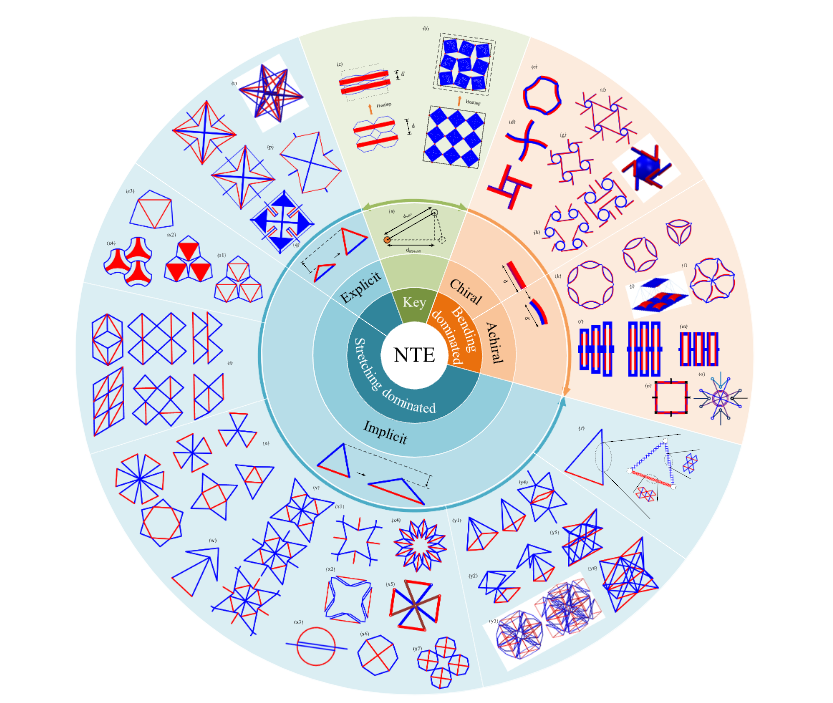
\includegraphics[width=0.79\linewidth]{Problem_5/Image/P5_I1.png}
    \caption{Một số cấu trúc NTE và đặc tính của nó được giới thiệu trong bài báo }
    \label{P5_I1}
\end{figure}

\vspace{0.5cm}

\noindent \textbf{\large Phổ điểm}
\begin{center}
\renewcommand{\arraystretch}{1.5}
\begin{tabularx}{\linewidth}{|c|X|c|}
\hline
\textbf{Phần} & \textbf{Nội dung} & \textbf{Điểm thành phần} \\ \hline
a & Thiết lập đúng biểu thức của $\Delta h$. & 0.5 \\ \cline{2-3} 
 & Tính đúng được $\alpha_{eff}$ từ $\Delta h \text{ và } h $. & 0.5 \\ \cline{2-3} 
 & Lập luận được các điều kiện của $\alpha_{eff}$. & 0.5 \\ \hline
b & Tính đúng tỉ số V'/V. & 1.0 \\ \hline
c & Thiết lập được thể tích trước và sau khi nở. & 0.5 \\ \cline{2-3} 
 & Biến đổi chuẩn tỉ số V'/V. & 0.5 \\ \cline{2-3} 
 & Thiết lập được hệ số nở khối hiệu dụng $\beta_{eff}$. & 0.5 \\ \hline
\multicolumn{2}{|r|}{\textbf{Tổng điểm}} & \textbf{4.0} \\ \hline
\end{tabularx}
\end{center}
